% Created by tikzDevice version 0.7.0 on 2014-08-02 16:07:02
% !TEX encoding = UTF-8 Unicode
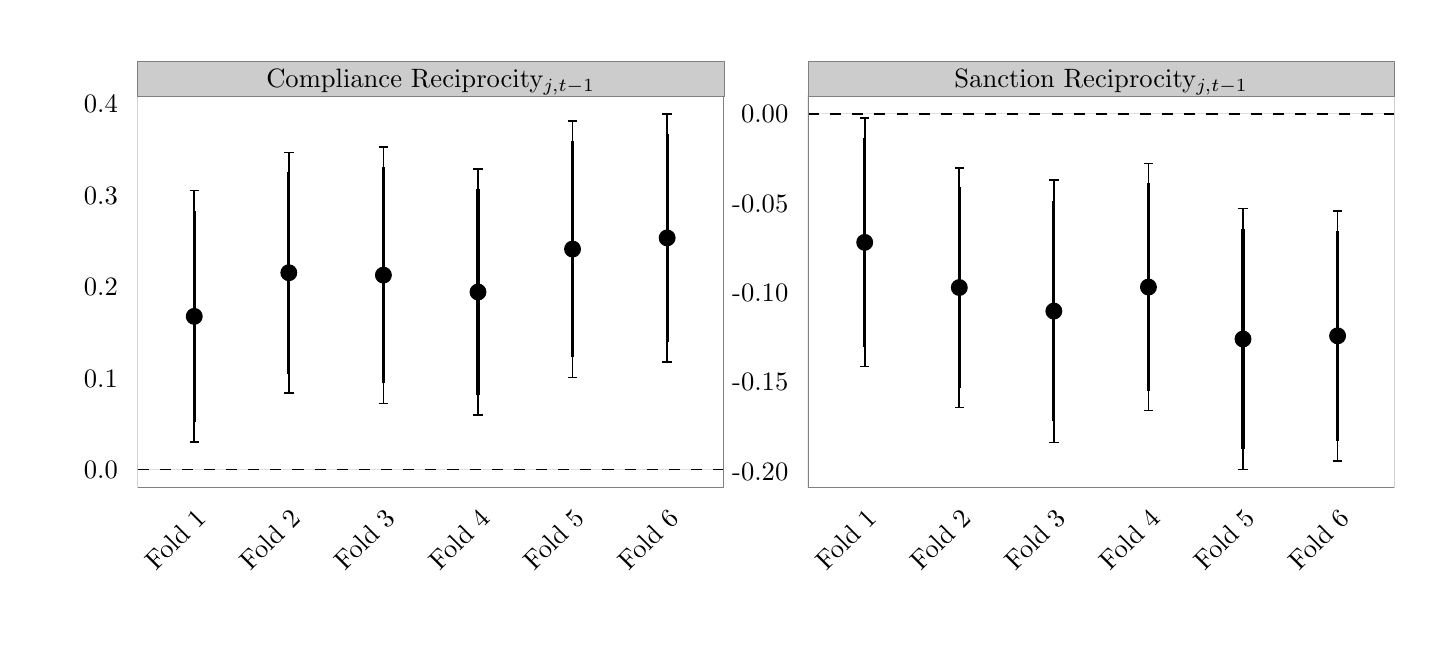
\begin{tikzpicture}[x=1pt,y=1pt]
\definecolor[named]{fillColor}{rgb}{1.00,1.00,1.00}
\path[use as bounding box,fill=fillColor,fill opacity=0.00] (0,0) rectangle (505.89,216.81);
\begin{scope}
\path[clip] (  0.00,  0.00) rectangle (505.89,216.81);
\definecolor[named]{drawColor}{rgb}{1.00,1.00,1.00}
\definecolor[named]{fillColor}{rgb}{1.00,1.00,1.00}

\path[draw=drawColor,line width= 0.6pt,line join=round,line cap=round,fill=fillColor] (  0.00,  0.00) rectangle (505.89,216.81);
\end{scope}
\begin{scope}
\path[clip] ( 39.69, 50.67) rectangle (251.57,192.13);
\definecolor[named]{fillColor}{rgb}{1.00,1.00,1.00}

\path[fill=fillColor] ( 39.69, 50.67) rectangle (251.57,192.13);
\definecolor[named]{drawColor}{rgb}{0.00,0.00,0.00}
\definecolor[named]{fillColor}{rgb}{0.00,0.00,0.00}

\path[draw=drawColor,draw opacity=0.30,line width= 0.3pt,line join=round,fill=fillColor,fill opacity=0.30] ( 60.19, 67.01) -- ( 60.19,157.97);

\path[draw=drawColor,draw opacity=0.30,line width= 0.3pt,line join=round,fill=fillColor,fill opacity=0.30] ( 94.37, 84.84) -- ( 94.37,171.68);

\path[draw=drawColor,draw opacity=0.30,line width= 0.3pt,line join=round,fill=fillColor,fill opacity=0.30] (128.54, 81.00) -- (128.54,173.77);

\path[draw=drawColor,draw opacity=0.30,line width= 0.3pt,line join=round,fill=fillColor,fill opacity=0.30] (162.72, 76.75) -- (162.72,165.85);

\path[draw=drawColor,draw opacity=0.30,line width= 0.3pt,line join=round,fill=fillColor,fill opacity=0.30] (196.89, 90.43) -- (196.89,183.18);

\path[draw=drawColor,draw opacity=0.30,line width= 0.3pt,line join=round,fill=fillColor,fill opacity=0.30] (231.07, 95.99) -- (231.07,185.70);
\definecolor[named]{drawColor}{rgb}{0.00,0.00,0.00}
\definecolor[named]{fillColor}{rgb}{0.00,0.00,0.00}

\path[draw=drawColor,line width= 1.1pt,line join=round,fill=fillColor] ( 60.19, 74.32) -- ( 60.19,150.66);

\path[draw=drawColor,line width= 1.1pt,line join=round,fill=fillColor] ( 94.37, 91.82) -- ( 94.37,164.70);

\path[draw=drawColor,line width= 1.1pt,line join=round,fill=fillColor] (128.54, 88.46) -- (128.54,166.31);

\path[draw=drawColor,line width= 1.1pt,line join=round,fill=fillColor] (162.72, 83.91) -- (162.72,158.69);

\path[draw=drawColor,line width= 1.1pt,line join=round,fill=fillColor] (196.89, 97.88) -- (196.89,175.73);

\path[draw=drawColor,line width= 1.1pt,line join=round,fill=fillColor] (231.07,103.20) -- (231.07,178.49);

\path[draw=drawColor,line width= 0.6pt,dash pattern=on 4pt off 4pt ,line join=round,fill=fillColor] ( 39.69, 57.10) -- (251.57, 57.10);

\path[draw=drawColor,line width= 0.4pt,line join=round,line cap=round,fill=fillColor] ( 60.19,112.49) circle (  2.85);

\path[draw=drawColor,line width= 0.4pt,line join=round,line cap=round,fill=fillColor] ( 94.37,128.26) circle (  2.85);

\path[draw=drawColor,line width= 0.4pt,line join=round,line cap=round,fill=fillColor] (128.54,127.39) circle (  2.85);

\path[draw=drawColor,line width= 0.4pt,line join=round,line cap=round,fill=fillColor] (162.72,121.30) circle (  2.85);

\path[draw=drawColor,line width= 0.4pt,line join=round,line cap=round,fill=fillColor] (196.89,136.80) circle (  2.85);

\path[draw=drawColor,line width= 0.4pt,line join=round,line cap=round,fill=fillColor] (231.07,140.84) circle (  2.85);

\path[draw=drawColor,line width= 0.6pt,line join=round] ( 58.48,157.97) --
	( 61.90,157.97);

\path[draw=drawColor,line width= 0.6pt,line join=round] ( 60.19,157.97) --
	( 60.19, 67.01);

\path[draw=drawColor,line width= 0.6pt,line join=round] ( 58.48, 67.01) --
	( 61.90, 67.01);

\path[draw=drawColor,line width= 0.6pt,line join=round] ( 92.66,171.68) --
	( 96.08,171.68);

\path[draw=drawColor,line width= 0.6pt,line join=round] ( 94.37,171.68) --
	( 94.37, 84.84);

\path[draw=drawColor,line width= 0.6pt,line join=round] ( 92.66, 84.84) --
	( 96.08, 84.84);

\path[draw=drawColor,line width= 0.6pt,line join=round] (126.83,173.77) --
	(130.25,173.77);

\path[draw=drawColor,line width= 0.6pt,line join=round] (128.54,173.77) --
	(128.54, 81.00);

\path[draw=drawColor,line width= 0.6pt,line join=round] (126.83, 81.00) --
	(130.25, 81.00);

\path[draw=drawColor,line width= 0.6pt,line join=round] (161.01,165.85) --
	(164.43,165.85);

\path[draw=drawColor,line width= 0.6pt,line join=round] (162.72,165.85) --
	(162.72, 76.75);

\path[draw=drawColor,line width= 0.6pt,line join=round] (161.01, 76.75) --
	(164.43, 76.75);

\path[draw=drawColor,line width= 0.6pt,line join=round] (195.18,183.18) --
	(198.60,183.18);

\path[draw=drawColor,line width= 0.6pt,line join=round] (196.89,183.18) --
	(196.89, 90.43);

\path[draw=drawColor,line width= 0.6pt,line join=round] (195.18, 90.43) --
	(198.60, 90.43);

\path[draw=drawColor,line width= 0.6pt,line join=round] (229.36,185.70) --
	(232.78,185.70);

\path[draw=drawColor,line width= 0.6pt,line join=round] (231.07,185.70) --
	(231.07, 95.99);

\path[draw=drawColor,line width= 0.6pt,line join=round] (229.36, 95.99) --
	(232.78, 95.99);
\definecolor[named]{drawColor}{rgb}{0.50,0.50,0.50}

\path[draw=drawColor,line width= 0.6pt,line join=round,line cap=round] ( 39.69, 50.67) rectangle (251.57,192.13);
\end{scope}
\begin{scope}
\path[clip] (281.96, 50.67) rectangle (493.85,192.13);
\definecolor[named]{fillColor}{rgb}{1.00,1.00,1.00}

\path[fill=fillColor] (281.96, 50.67) rectangle (493.85,192.13);
\definecolor[named]{drawColor}{rgb}{0.00,0.00,0.00}
\definecolor[named]{fillColor}{rgb}{0.00,0.00,0.00}

\path[draw=drawColor,draw opacity=0.30,line width= 0.3pt,line join=round,fill=fillColor,fill opacity=0.30] (302.46, 94.34) -- (302.46,184.13);

\path[draw=drawColor,draw opacity=0.30,line width= 0.3pt,line join=round,fill=fillColor,fill opacity=0.30] (336.64, 79.61) -- (336.64,166.21);

\path[draw=drawColor,draw opacity=0.30,line width= 0.3pt,line join=round,fill=fillColor,fill opacity=0.30] (370.81, 66.95) -- (370.81,161.82);

\path[draw=drawColor,draw opacity=0.30,line width= 0.3pt,line join=round,fill=fillColor,fill opacity=0.30] (404.99, 78.48) -- (404.99,167.69);

\path[draw=drawColor,draw opacity=0.30,line width= 0.3pt,line join=round,fill=fillColor,fill opacity=0.30] (439.16, 57.10) -- (439.16,151.50);

\path[draw=drawColor,draw opacity=0.30,line width= 0.3pt,line join=round,fill=fillColor,fill opacity=0.30] (473.34, 60.25) -- (473.34,150.65);
\definecolor[named]{drawColor}{rgb}{0.00,0.00,0.00}
\definecolor[named]{fillColor}{rgb}{0.00,0.00,0.00}

\path[draw=drawColor,line width= 1.1pt,line join=round,fill=fillColor] (302.46,101.55) -- (302.46,176.91);

\path[draw=drawColor,line width= 1.1pt,line join=round,fill=fillColor] (336.64, 86.57) -- (336.64,159.25);

\path[draw=drawColor,line width= 1.1pt,line join=round,fill=fillColor] (370.81, 74.58) -- (370.81,154.20);

\path[draw=drawColor,line width= 1.1pt,line join=round,fill=fillColor] (404.99, 85.65) -- (404.99,160.52);

\path[draw=drawColor,line width= 1.1pt,line join=round,fill=fillColor] (439.16, 64.69) -- (439.16,143.91);

\path[draw=drawColor,line width= 1.1pt,line join=round,fill=fillColor] (473.34, 67.52) -- (473.34,143.38);

\path[draw=drawColor,line width= 0.6pt,dash pattern=on 4pt off 4pt ,line join=round,fill=fillColor] (281.96,185.70) -- (493.85,185.70);

\path[draw=drawColor,line width= 0.4pt,line join=round,line cap=round,fill=fillColor] (302.46,139.23) circle (  2.85);

\path[draw=drawColor,line width= 0.4pt,line join=round,line cap=round,fill=fillColor] (336.64,122.91) circle (  2.85);

\path[draw=drawColor,line width= 0.4pt,line join=round,line cap=round,fill=fillColor] (370.81,114.39) circle (  2.85);

\path[draw=drawColor,line width= 0.4pt,line join=round,line cap=round,fill=fillColor] (404.99,123.08) circle (  2.85);

\path[draw=drawColor,line width= 0.4pt,line join=round,line cap=round,fill=fillColor] (439.16,104.30) circle (  2.85);

\path[draw=drawColor,line width= 0.4pt,line join=round,line cap=round,fill=fillColor] (473.34,105.45) circle (  2.85);

\path[draw=drawColor,line width= 0.6pt,line join=round] (300.76,184.13) --
	(304.17,184.13);

\path[draw=drawColor,line width= 0.6pt,line join=round] (302.46,184.13) --
	(302.46, 94.34);

\path[draw=drawColor,line width= 0.6pt,line join=round] (300.76, 94.34) --
	(304.17, 94.34);

\path[draw=drawColor,line width= 0.6pt,line join=round] (334.93,166.21) --
	(338.35,166.21);

\path[draw=drawColor,line width= 0.6pt,line join=round] (336.64,166.21) --
	(336.64, 79.61);

\path[draw=drawColor,line width= 0.6pt,line join=round] (334.93, 79.61) --
	(338.35, 79.61);

\path[draw=drawColor,line width= 0.6pt,line join=round] (369.11,161.82) --
	(372.52,161.82);

\path[draw=drawColor,line width= 0.6pt,line join=round] (370.81,161.82) --
	(370.81, 66.95);

\path[draw=drawColor,line width= 0.6pt,line join=round] (369.11, 66.95) --
	(372.52, 66.95);

\path[draw=drawColor,line width= 0.6pt,line join=round] (403.28,167.69) --
	(406.70,167.69);

\path[draw=drawColor,line width= 0.6pt,line join=round] (404.99,167.69) --
	(404.99, 78.48);

\path[draw=drawColor,line width= 0.6pt,line join=round] (403.28, 78.48) --
	(406.70, 78.48);

\path[draw=drawColor,line width= 0.6pt,line join=round] (437.46,151.50) --
	(440.87,151.50);

\path[draw=drawColor,line width= 0.6pt,line join=round] (439.16,151.50) --
	(439.16, 57.10);

\path[draw=drawColor,line width= 0.6pt,line join=round] (437.46, 57.10) --
	(440.87, 57.10);

\path[draw=drawColor,line width= 0.6pt,line join=round] (471.63,150.65) --
	(475.05,150.65);

\path[draw=drawColor,line width= 0.6pt,line join=round] (473.34,150.65) --
	(473.34, 60.25);

\path[draw=drawColor,line width= 0.6pt,line join=round] (471.63, 60.25) --
	(475.05, 60.25);
\definecolor[named]{drawColor}{rgb}{0.50,0.50,0.50}

\path[draw=drawColor,line width= 0.6pt,line join=round,line cap=round] (281.96, 50.67) rectangle (493.85,192.13);
\end{scope}
\begin{scope}
\path[clip] (  0.00,  0.00) rectangle (505.89,216.81);
\definecolor[named]{drawColor}{rgb}{0.50,0.50,0.50}
\definecolor[named]{fillColor}{rgb}{0.80,0.80,0.80}

\path[draw=drawColor,line width= 0.2pt,line join=round,line cap=round,fill=fillColor] ( 39.69,192.13) rectangle (251.57,204.77);
\definecolor[named]{drawColor}{rgb}{0.00,0.00,0.00}

\node[text=drawColor,anchor=base,inner sep=0pt, outer sep=0pt, scale=  0.96] at (145.63,195.14) {Compliance Reciprocity$_{j,t-1}$};
\end{scope}
\begin{scope}
\path[clip] (  0.00,  0.00) rectangle (505.89,216.81);
\definecolor[named]{drawColor}{rgb}{0.50,0.50,0.50}
\definecolor[named]{fillColor}{rgb}{0.80,0.80,0.80}

\path[draw=drawColor,line width= 0.2pt,line join=round,line cap=round,fill=fillColor] (281.96,192.13) rectangle (493.85,204.77);
\definecolor[named]{drawColor}{rgb}{0.00,0.00,0.00}

\node[text=drawColor,anchor=base,inner sep=0pt, outer sep=0pt, scale=  0.96] at (387.90,195.14) {Sanction Reciprocity$_{j,t-1}$};
\end{scope}
\begin{scope}
\path[clip] (  0.00,  0.00) rectangle (505.89,216.81);
\definecolor[named]{drawColor}{rgb}{0.00,0.00,0.00}

\node[text=drawColor,anchor=base east,inner sep=0pt, outer sep=0pt, scale=  0.96] at ( 32.57, 53.79) {0.0};

\node[text=drawColor,anchor=base east,inner sep=0pt, outer sep=0pt, scale=  0.96] at ( 32.57, 86.88) {0.1};

\node[text=drawColor,anchor=base east,inner sep=0pt, outer sep=0pt, scale=  0.96] at ( 32.57,119.97) {0.2};

\node[text=drawColor,anchor=base east,inner sep=0pt, outer sep=0pt, scale=  0.96] at ( 32.57,153.05) {0.3};

\node[text=drawColor,anchor=base east,inner sep=0pt, outer sep=0pt, scale=  0.96] at ( 32.57,186.14) {0.4};
\end{scope}
\begin{scope}
\path[clip] (  0.00,  0.00) rectangle (505.89,216.81);
\definecolor[named]{drawColor}{rgb}{0.00,0.00,0.00}

\node[text=drawColor,anchor=base east,inner sep=0pt, outer sep=0pt, scale=  0.96] at (274.85, 53.29) {-0.20};

\node[text=drawColor,anchor=base east,inner sep=0pt, outer sep=0pt, scale=  0.96] at (274.85, 85.57) {-0.15};

\node[text=drawColor,anchor=base east,inner sep=0pt, outer sep=0pt, scale=  0.96] at (274.85,117.84) {-0.10};

\node[text=drawColor,anchor=base east,inner sep=0pt, outer sep=0pt, scale=  0.96] at (274.85,150.12) {-0.05};

\node[text=drawColor,anchor=base east,inner sep=0pt, outer sep=0pt, scale=  0.96] at (274.85,182.39) {0.00};
\end{scope}
\begin{scope}
\path[clip] (  0.00,  0.00) rectangle (505.89,216.81);
\definecolor[named]{drawColor}{rgb}{0.00,0.00,0.00}

\node[text=drawColor,rotate= 45.00,anchor=base east,inner sep=0pt, outer sep=0pt, scale=  0.96] at ( 64.87, 38.88) {Fold 1};

\node[text=drawColor,rotate= 45.00,anchor=base east,inner sep=0pt, outer sep=0pt, scale=  0.96] at ( 99.04, 38.88) {Fold 2};

\node[text=drawColor,rotate= 45.00,anchor=base east,inner sep=0pt, outer sep=0pt, scale=  0.96] at (133.22, 38.88) {Fold 3};

\node[text=drawColor,rotate= 45.00,anchor=base east,inner sep=0pt, outer sep=0pt, scale=  0.96] at (167.39, 38.88) {Fold 4};

\node[text=drawColor,rotate= 45.00,anchor=base east,inner sep=0pt, outer sep=0pt, scale=  0.96] at (201.57, 38.88) {Fold 5};

\node[text=drawColor,rotate= 45.00,anchor=base east,inner sep=0pt, outer sep=0pt, scale=  0.96] at (235.74, 38.88) {Fold 6};
\end{scope}
\begin{scope}
\path[clip] (  0.00,  0.00) rectangle (505.89,216.81);
\definecolor[named]{drawColor}{rgb}{0.00,0.00,0.00}

\node[text=drawColor,rotate= 45.00,anchor=base east,inner sep=0pt, outer sep=0pt, scale=  0.96] at (307.14, 38.88) {Fold 1};

\node[text=drawColor,rotate= 45.00,anchor=base east,inner sep=0pt, outer sep=0pt, scale=  0.96] at (341.31, 38.88) {Fold 2};

\node[text=drawColor,rotate= 45.00,anchor=base east,inner sep=0pt, outer sep=0pt, scale=  0.96] at (375.49, 38.88) {Fold 3};

\node[text=drawColor,rotate= 45.00,anchor=base east,inner sep=0pt, outer sep=0pt, scale=  0.96] at (409.66, 38.88) {Fold 4};

\node[text=drawColor,rotate= 45.00,anchor=base east,inner sep=0pt, outer sep=0pt, scale=  0.96] at (443.84, 38.88) {Fold 5};

\node[text=drawColor,rotate= 45.00,anchor=base east,inner sep=0pt, outer sep=0pt, scale=  0.96] at (478.02, 38.88) {Fold 6};
\end{scope}
\end{tikzpicture}
